\documentclass[12pt,a4paper]{article}

% --- Packages ---
\usepackage[utf8]{inputenc}
\usepackage[T1]{fontenc}
\usepackage[english]{babel}
\usepackage{geometry}
\geometry{margin=2.5cm, headheight=14pt}
\usepackage{graphicx}
\usepackage{amsmath,amssymb}
\usepackage{booktabs}
\usepackage{caption}
\usepackage{subcaption}
\usepackage{hyperref}
\usepackage{listings}
\usepackage{xcolor}
\usepackage{float}
\usepackage{enumitem}
\usepackage{array}
\usepackage{tabularx}
\usepackage{fancyhdr}
\usepackage{titlesec}
\usepackage{appendix}

% --- Code Listing Style ---
\lstdefinestyle{pythonstyle}{
    language=Python,
    basicstyle=\ttfamily\small,
    keywordstyle=\color{blue}\bfseries,
    commentstyle=\color{gray}\itshape,
    stringstyle=\color{orange},
    numberstyle=\tiny\color{gray},
    numbers=left,
    numbersep=5pt,
    breaklines=true,
    frame=single,
    backgroundcolor=\color{gray!5},
    captionpos=b,
    tabsize=4
}

% --- Header/Footer ---
\pagestyle{fancy}
\fancyhf{}
\fancyhead[L]{\small Assignment 3 -- Distraction Monitoring}
\fancyhead[R]{\small Jacopo Rialti -- s346357}
\fancyfoot[C]{\thepage}

% --- Hyperref Setup ---
\hypersetup{
    colorlinks=true,
    linkcolor=blue!70!black,
    citecolor=blue!70!black,
    urlcolor=blue!70!black
}

% --- Title ---
\title{
    \vspace{-1cm}
    \textbf{Assignment 3: Distraction Monitoring} \\[0.3cm]
    \large Technologies for Autonomous Vehicles (T4AV) \\
    Politecnico di Torino
}
\author{
    Jacopo Rialti -- s346357
}

\begin{document}

\maketitle
\thispagestyle{fancy}



\tableofcontents
\newpage

% ============================================================
% APPENDIX -- placed at the beginning as requested
% ============================================================
% Appendix is placed at the end -- see below
% Table of contents follows


% ============================================================
% 1. INTRODUCTION
% ============================================================
\section{Introduction}\label{sec:intro}

Driver distraction and drowsiness are among the leading causes of road accidents worldwide. Advanced Driver Assistance Systems (ADAS) increasingly incorporate Driver Monitoring Systems to detect unsafe driver behaviour and issue timely warnings. The objective of this assignment is to implement a DMS using a standard laptop webcam and computer vision techniques.

The implemented system, contained in the top-level script \texttt{runDMS.py}, processes the webcam video stream in real time and identifies the following critical conditions:

\begin{itemize}[noitemsep]
    \item \textbf{Long Owl Distraction} (mandatory): the driver head is turned away from the forward road for at least 5 continuous seconds.
    \item \textbf{Short Owl Distraction} (mandatory): the driver head turns away from the road and back repeatedly, accumulating 10 seconds of off-road gaze within a 30-second sliding window.
    \item \textbf{Long Lizard Distraction} (optional): the driver head remains forward but the eyes gaze sideways for at least 5 continuous seconds.
    \item \textbf{Short Lizard Distraction} (optional): same cumulative criterion as short owl, but applied to eye gaze while the head remains centred.
    \item \textbf{Microsleep Warning} (mandatory): both eyes remain closed for at least 4 seconds.
    \item \textbf{Sleep Warning} (mandatory): both eyes remain closed for at least 7 seconds.
    \item \textbf{Heart Rate Display} (mandatory): the driver heart rate in beats per minute (BPM) is estimated via remote photoplethysmography and displayed on screen.
\end{itemize}

The output is a live video of the driver face with the current state displayed in the bottom-right corner and the estimated heart rate displayed in the bottom-left corner, in accordance with the assignment specifications.

% ============================================================
% 2. METHODOLOGY
% ============================================================
\section{Methodology}\label{sec:method}

This section provides a detailed description of each technique employed in the DMS, the rationale behind every design choice, and how the implementation relates to the examples provided by the instructor.

% --- 2.1 Face Detection and Landmark Extraction ---
\subsection{Face Detection and Landmark Extraction}\label{subsec:face}

The system employs the \textbf{MediaPipe Face Mesh} model to detect and track 478 three-dimensional facial landmarks in real time. 


The Face Mesh is configured with:
\begin{itemize}[noitemsep]
    \item \texttt{max\_num\_faces = 1}: only one driver face is expected.
    \item \texttt{refine\_landmarks = True}: enables the iris landmark refinement model, which provides 10 additional landmarks for the left and right iris (indices 468--477). This is essential for the lizard distraction detection.
    \item \texttt{min\_detection\_confidence = 0.5} and \texttt{min\_tracking\_confidence = 0.5}: standard thresholds.
\end{itemize}

Each frame is horizontally flipped to produce a selfie-view (mirrored) display, converted from BGR to RGB for MediaPipe processing, and then processed to extract the landmark array. Relevant landmarks are then used to compute the geometric features described in the following subsections.

% --- 2.2 Eye Aspect Ratio ---
\subsection{Eye Aspect Ratio (EAR) for Drowsiness Detection}\label{subsec:ear}

To detect whether the driver eyes are open or closed, the system computes the \textbf{Eye Aspect Ratio (EAR)}, a well-established metric in the literature. The EAR is defined as:

\begin{equation}\label{eq:ear}
    \text{EAR} = \frac{\|p_2 - p_6\| + \|p_3 - p_5\|}{2 \cdot \|p_1 - p_4\|}
\end{equation}

\noindent where $p_1, \ldots, p_6$ are six specific landmarks around each eye. The numerator captures the vertical opening of the eye (two vertical distances), while the denominator captures the horizontal extent. When the eye is open, the EAR assumes values around 0.25--0.35; when the eye is closed, the vertical distances collapse and the EAR drops below 0.20.

The landmark indices used are:
\begin{itemize}[noitemsep]
    \item \textbf{Left eye}: 33, 160, 158, 133, 153, 144
    \item \textbf{Right eye}: 362, 385, 387, 263, 373, 380
\end{itemize}

These indices were selected from the MediaPipe Face Mesh topology to capture the inner corner, outer corner, and the upper and lower eyelid midpoints for each eye. The average EAR of both eyes is computed to produce a single, more robust estimate. A threshold of $\text{EAR}_{\text{thresh}} = 0.20$ is used to classify the eye state as closed.

% --- 2.3 Head Yaw Ratio ---
\subsection{Head Yaw Ratio for Owl Distraction}\label{subsec:headyaw}

To estimate whether the driver head is turned away from the forward road, the system computes a \textbf{head yaw ratio} based on the relative horizontal position of the nose tip with respect to the left and right cheek landmarks.

The head yaw ratio is defined as:

\begin{equation}\label{eq:headyaw}
    r_{\text{head}} = \frac{d(\text{nose}, \text{left cheek})}{d(\text{nose}, \text{left cheek}) + d(\text{nose}, \text{right cheek})}
\end{equation}

\noindent where $d(\cdot, \cdot)$ denotes the Euclidean distance in image coordinates. The landmarks used are:
\begin{itemize}[noitemsep]
    \item \textbf{Nose tip}: index 1
    \item \textbf{Left cheek}: index 234
    \item \textbf{Right cheek}: index 454
\end{itemize}

When the driver looks straight ahead, the nose is roughly equidistant from both cheeks, yielding $r_{\text{head}} \approx 0.5$. When the head rotates to the left, the nose moves closer to the left cheek and $r_{\text{head}}$ decreases; conversely, a right rotation increases $r_{\text{head}}$. The system flags head distraction when $|r_{\text{head}} - 0.5| > 0.20$, meaning the ratio deviates by more than 0.20 from the neutral position.

% --- 2.4 Eye Yaw Ratio ---
\subsection{Eye Yaw Ratio for Lizard Distraction}\label{subsec:eyeyaw}

The lizard distraction requires detecting lateral eye gaze while the head remains centred. The system computes an \textbf{eye yaw ratio} that measures the horizontal position of the iris centre relative to the eye corners:

\begin{equation}\label{eq:eyeyaw}
    r_{\text{eye}} = \frac{|x_{\text{iris}} - x_{\text{inner}}|}{|x_{\text{iris}} - x_{\text{inner}}| + |x_{\text{iris}} - x_{\text{outer}}|}
\end{equation}

\noindent where $x_{\text{iris}}$, $x_{\text{inner}}$, and $x_{\text{outer}}$ are the horizontal pixel coordinates of the iris centre, the inner eye corner, and the outer eye corner, respectively. Only the $x$-coordinate is used because the $z$-coordinate provided by MediaPipe proved to be excessively noisy for this application.

The iris centre landmarks (473 for the left eye and 468 for the right eye) are available only when \texttt{refine\_landmarks = True} is enabled, as in our configuration. The ratio for both eyes is averaged.

A critical design choice is the use of a \textbf{dynamic baseline} instead of a hardcoded value of 0.5. In practice, the resting iris position varies across individuals and camera setups. Therefore, the system maintains a slowly adapting baseline using a very slow EMA ($\alpha = 0.002$):

\begin{equation}
    b_{\text{eye}}^{(t)} = 0.002 \cdot \bar{r}_{\text{eye}}^{(t)} + 0.998 \cdot b_{\text{eye}}^{(t-1)}
\end{equation}

This baseline is updated only when the head is confirmed to be in a strictly centred position ($|r_{\text{head}} - 0.5| < 0.10$), ensuring that only forward-looking samples contribute. The lizard distraction is flagged when $|r_{\text{eye}} - b_{\text{eye}}| > 0.006$ and the head is strictly centred. The low threshold reflects the fact that iris movements produce smaller ratio changes than head movements.

% --- 2.5 Signal Smoothing ---
\subsection{Signal Smoothing with Exponential Moving Average}\label{subsec:ema}

Raw landmark coordinates from frame-to-frame exhibit considerable jitter due to detection noise, sub-pixel inaccuracies, and minor involuntary facial movements. Without smoothing, this noise causes rapid oscillations in the computed ratios, which in turn lead to erratic toggling of distraction flags and premature resetting of timers.

To address this, an \textbf{Exponential Moving Average (EMA)} filter is applied to all three signals (EAR, head yaw ratio, eye yaw ratio):

\begin{equation}\label{eq:ema}
    \hat{s}^{(t)} = \alpha \cdot s^{(t)} + (1 - \alpha) \cdot \hat{s}^{(t-1)}
\end{equation}

\noindent where $s^{(t)}$ is the raw measurement at time $t$, $\hat{s}^{(t)}$ is the smoothed value, and $\alpha = 0.15$ is the smoothing coefficient. This value of $\alpha$ was chosen empirically as a trade-off between responsiveness and stability: a lower $\alpha$ would over-smooth and delay detection, whereas a higher $\alpha$ would not sufficiently suppress noise.

The EMA filter was preferred over other alternatives (e.g., moving average, Gaussian filter) because it requires no buffer of past samples, is computationally trivial, and naturally gives exponentially decaying weight to older measurements.


% --- 2.6 Distraction State Machine --- 

The core logic of the DMS is a \textbf{state machine} that maps the instantaneous signals to one of the following mutually exclusive driver states:

\begin{enumerate}[noitemsep]
    \item \textbf{Sleep}: eyes closed for $\geq 7$ seconds continuously. Cleared when eyes are open for $\geq 2$ seconds.
    \item \textbf{Microsleep}: eyes closed for $\geq 4$ seconds continuously (and sleep not active). Cleared when eyes open for $\geq 2$ seconds.
    \item \textbf{Long Owl}: head continuously turned away for $\geq 5$ seconds. Cleared when head returns forward.
    \item \textbf{Long Lizard}: eyes continuously gazing sideways (head centred) for $\geq 5$ seconds. Cleared when eyes return forward.
    \item \textbf{Short Owl}: cumulative head-away time $\geq 10$ seconds within a 30-second sliding window. Cleared when head is forward for $\geq 2$ seconds.
    \item \textbf{Short Lizard}: cumulative eyes-away time $\geq 10$ seconds within a 30-second sliding window. Cleared when eyes are forward for $\geq 2$ seconds.
    \item \textbf{Focused on the road}: none of the above conditions are met.
\end{enumerate}

States are evaluated in priority order (Sleep $>$ Microsleep $>$ Long Owl $>$ Long Lizard $>$ Short Owl $>$ Short Lizard $>$ Focused), and only the highest-priority active state is displayed.

\subsubsection{Continuous Event Tracking}

For the long distractions and drowsiness events, the system tracks the last time the driver was in a ``safe'' state. For example, \texttt{last\_head\_forward\_time} records the most recent time the head was facing forward. However, to prevent noise-induced micro-resets, the system requires the head to remain forward for at least 0.5 seconds before updating this timer. This debouncing mechanism is critical: without it, a single noisy frame where the head momentarily appears forward would reset the entire distraction timer.

\subsubsection{Cumulative Time Calculation}

For the short distractions, a \textbf{sliding window} approach is used. A deque stores timestamped boolean entries indicating whether the driver was distracted at each frame. Entries older than 30 seconds are continuously removed. The cumulative distraction time is computed by summing the time intervals during which the distracted flag was true:

\begin{equation}
    T_{\text{cum}} = \sum_{i=1}^{N-1} (t_{i+1} - t_i) \cdot \mathbb{1}[\text{distracted}_i = \text{true}]
\end{equation}

When the short distraction state is cleared (after 2 seconds of forward gaze), the history deque is also cleared to prevent immediate re-triggering.

% --- 2.7 Heart Rate Estimation ---
\subsection{Heart Rate Estimation via Remote Photoplethysmography}\label{subsec:rppg}

The system estimates the driver heart rate using \textbf{remote photoplethysmography (rPPG)}. The key idea is that blood volume changes caused by the cardiac cycle produce subtle colour variations on the skin surface, which can be captured by a standard camera.

\subsubsection{Region of Interest Extraction}

The face silhouette defined by 36 MediaPipe landmarks is used as the Region of Interest (ROI). For each frame, a convex polygon mask is created from these landmarks, and the mean R, G, and B values within the mask are computed. These values are appended to circular buffers of length 300 (approximately 10 seconds of video at 30 fps).

\subsubsection{Signal Processing Pipeline}

The rPPG pipeline consists of the following steps:

\begin{enumerate}[noitemsep]
    \item \textbf{Bandpass Filtering}: A 3rd-order Butterworth bandpass filter with cutoff frequencies of 0.75\,Hz (45\,BPM) and 2.75\,Hz (165\,BPM) is applied to the R, G, and B time series. This removes DC drift and high-frequency noise while retaining the physiologically plausible heart rate range.
    
    \item \textbf{Independent Component Analysis (ICA)}: The three filtered colour channels are stacked into a matrix $\mathbf{X} \in \mathbb{R}^{N \times 3}$ and decomposed using the \textbf{FastICA} algorithm. This step aims to deconvolve the observed RGB variations into three independent source signals, based on the assumption that the cardiac pulse, motion artefacts, and illumination changes are statistically independent. This approach allows the isolation of the plethysmographic signal into one of the components, providing a robust method for extracting the periodic blood volume pulse from non-cardiac noise.
    
    \item \textbf{Frequency Analysis}: For each of the three independent components, the power spectral density is computed via the Fast Fourier Transform (FFT). The frequency bin with the maximum power within the valid heart rate range (0.75--2.75\,Hz) is identified, and the corresponding frequency is converted to BPM ($\text{HR} = f_{\text{peak}} \times 60$).
    
    \item \textbf{Component Selection}: The component whose peak frequency has the highest spectral power is selected as the best estimate of the cardiac signal.
\end{enumerate}

The heart rate is updated every 1 second to avoid excessive computational load, and at least 100 frames must be collected before the first estimate is produced. The estimated FPS is computed dynamically from the timestamp buffer to ensure correct frequency-domain scaling.

% ============================================================
% 3. PARAMETER SELECTION
% ============================================================
\section{Parameter Selection}\label{sec:params}

Table~\ref{tab:params} summarises all configurable parameters and their chosen values, along with the rationale for each choice.

\begin{table}[H]
\centering
\caption{Summary of system parameters and their justification.}
\label{tab:params}
\small
\begin{tabularx}{\textwidth}{l c X}
\toprule
\textbf{Parameter} & \textbf{Value} & \textbf{Rationale} \\
\midrule
EAR threshold & 0.20 & Standard value from the literature; empirically validated to reliably distinguish open from closed eyes. \\
Head yaw threshold & 0.20 & Allows moderate head turns without triggering; captures clear lateral turns. \\
Iris yaw threshold & 0.006 & Very small because iris-to-corner ratio changes are subtle compared to head movements. \\
Strict head centre threshold & 0.10 & Ensures lizard detection only activates when the head is genuinely forward-facing. \\
EMA coefficient ($\alpha$) & 0.15 & Balances noise suppression with responsiveness; tested values from 0.05 to 0.30. \\
Baseline EMA ($\alpha_b$) & 0.002 & Very slow adaptation prevents the baseline from drifting during lateral gaze. \\
Debounce duration & 0.5\,s & Prevents noise spikes from resetting continuous distraction timers. \\
rPPG buffer length & 300 & Approx.\ 10\,s at 30\,fps; provides sufficient frequency resolution for HR estimation. \\
Bandpass low cutoff & 0.75\,Hz & Corresponds to 45\,BPM (lower physiological bound). \\
Bandpass high cutoff & 2.75\,Hz & Corresponds to 165\,BPM (upper physiological bound during stress). \\
Butterworth order & 3 & Provides adequate roll-off without excessive phase distortion. \\
\bottomrule
\end{tabularx}
\end{table}

% ============================================================
% 4. VISUAL RESULTS
% ============================================================
\section{Visual Results}\label{sec:results}

The DMS was tested across all possible driver states. Table~\ref{tab:screenshots} presents representative screenshots captured during operation. Each screenshot shows the live webcam feed with the driver state label (bottom-right) and heart rate estimate (bottom-left) overlaid, along with debug information (top-left) displaying the real-time values of the eye yaw, head yaw, and EAR metrics.

\begin{table}[H]
\centering
\caption{Screenshots of the DMS output for each detected driver state.}
\label{tab:screenshots}
\small
\begin{tabular}{>{\centering\arraybackslash}m{0.45\textwidth} >{\centering\arraybackslash}m{0.45\textwidth}}
\toprule
\textbf{State} & \textbf{State} \\
\midrule
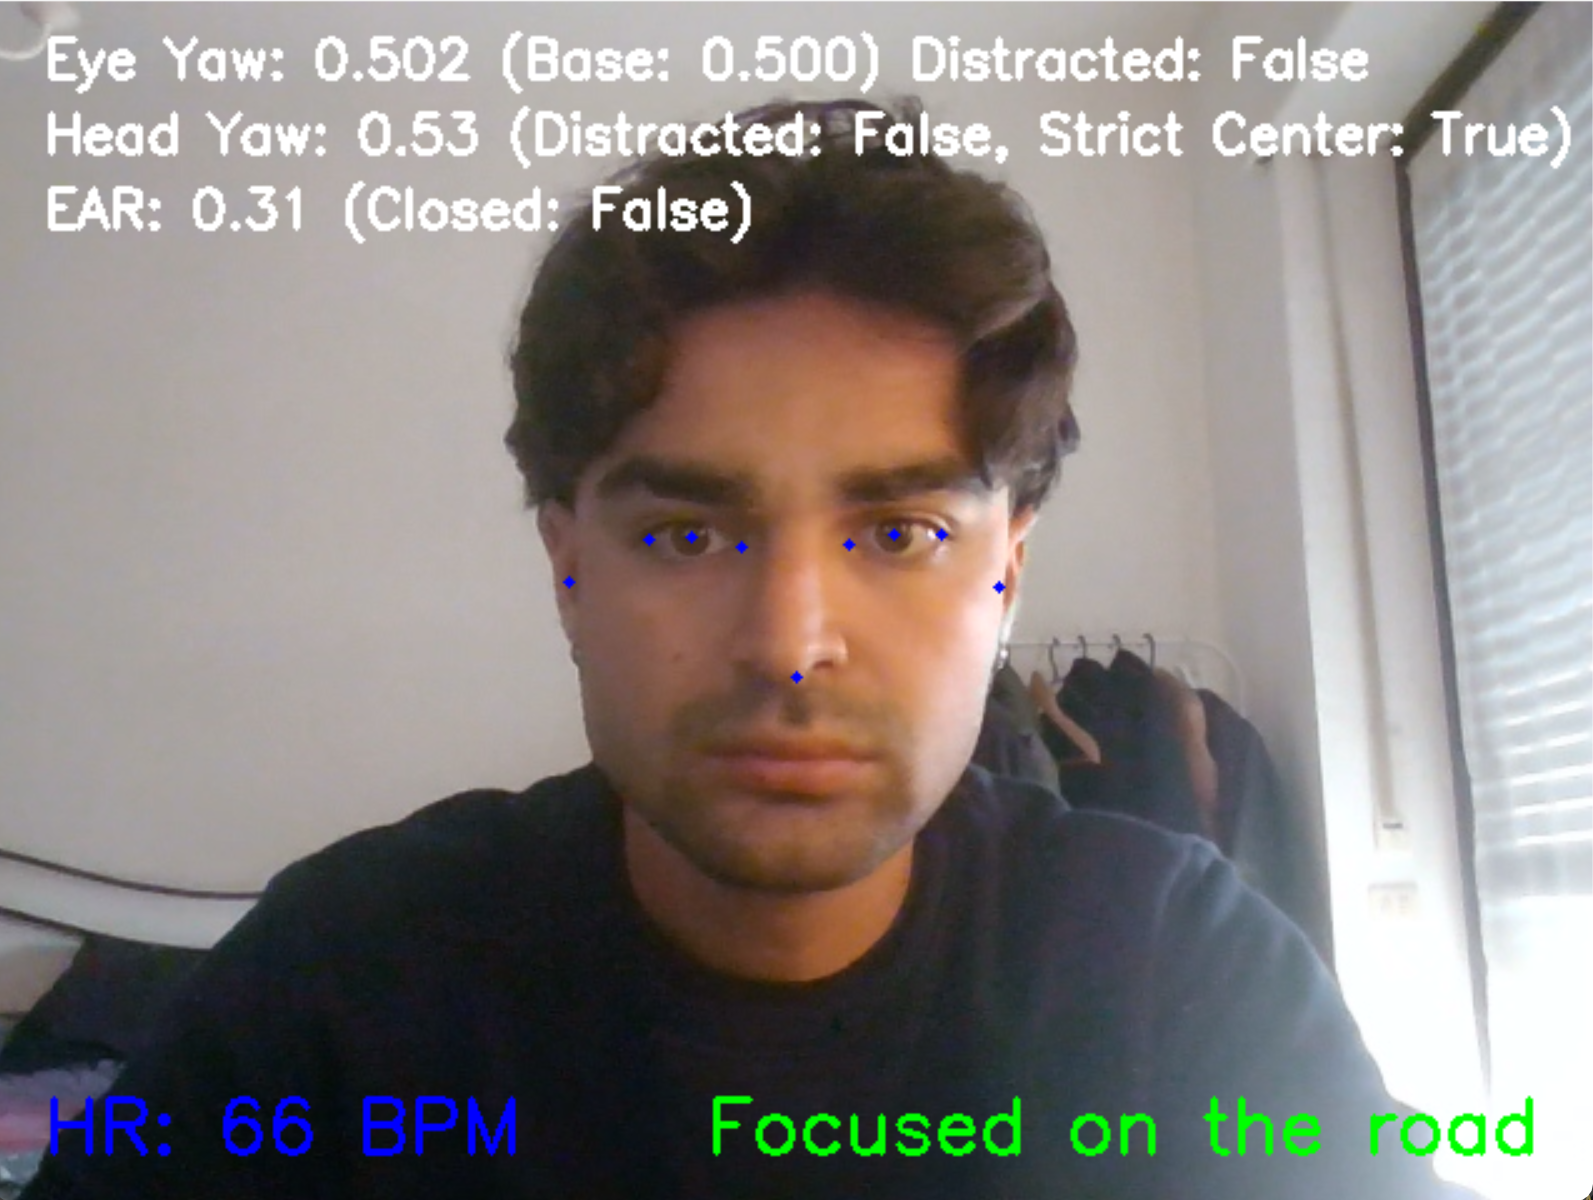
\includegraphics[width=0.42\textwidth]{images/focus_road.png} &
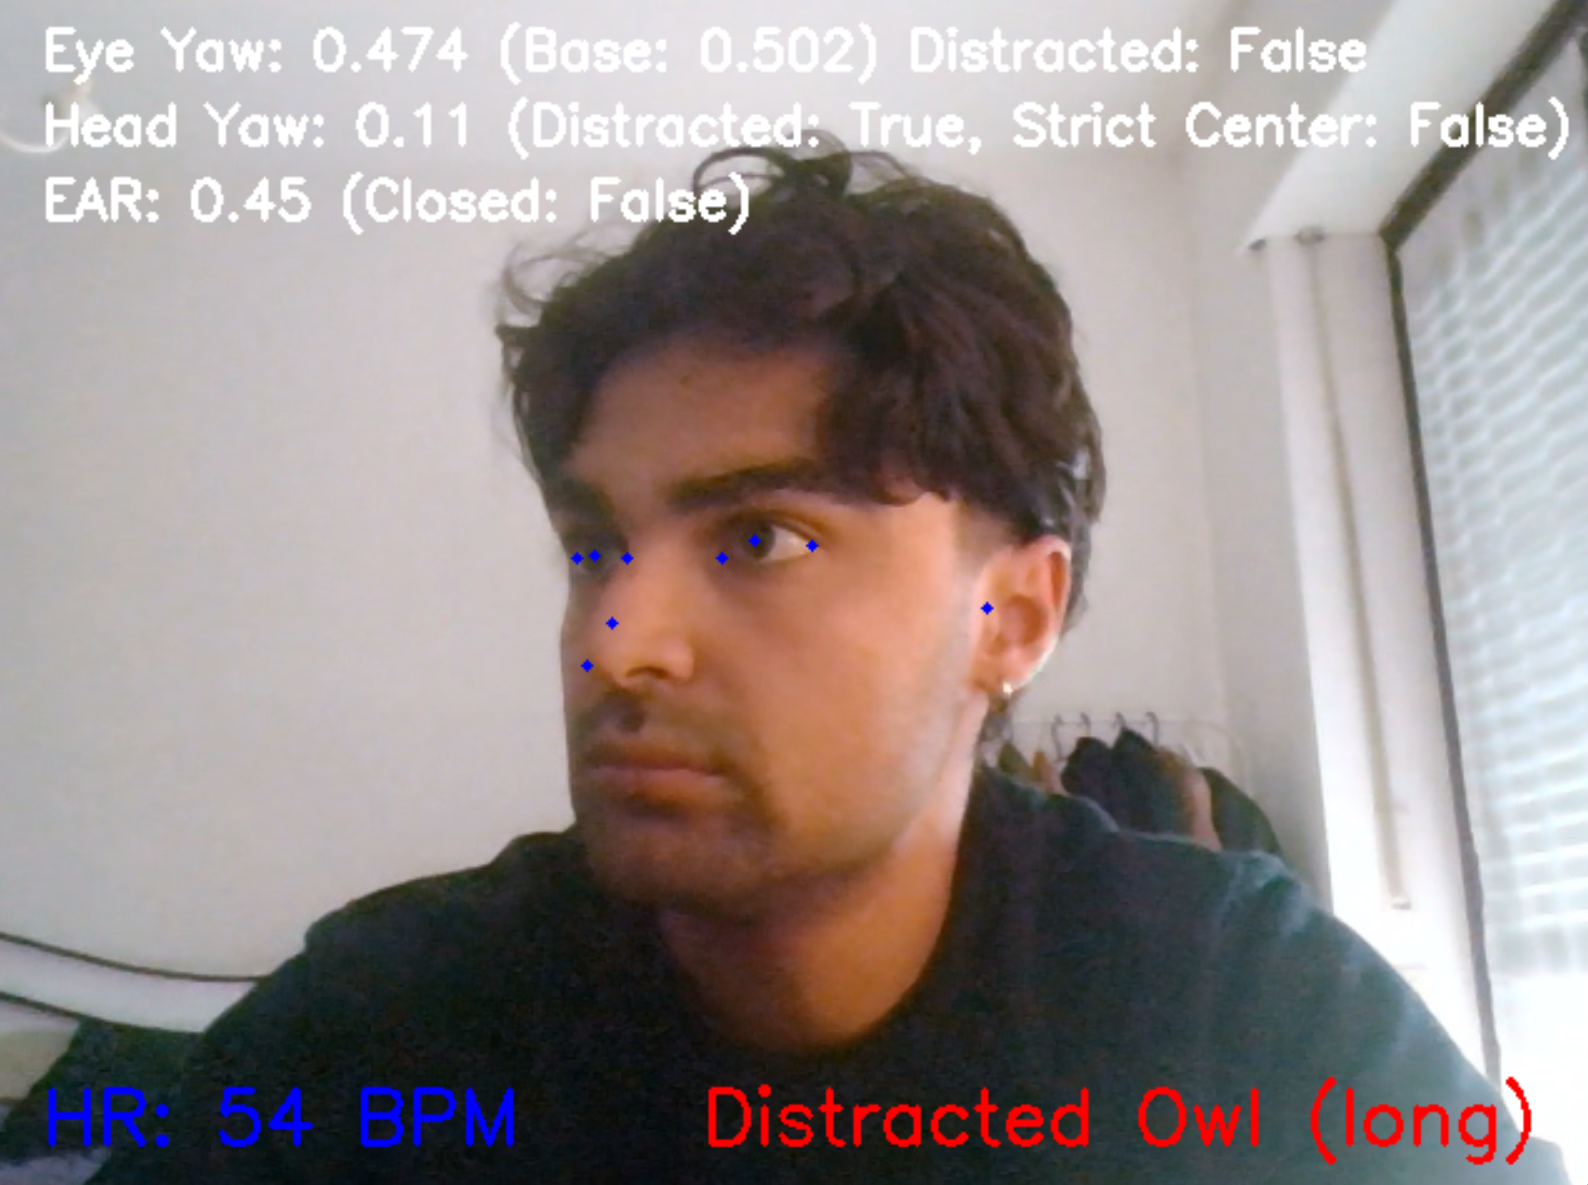
\includegraphics[width=0.42\textwidth]{images/distracted_owl_long.png} \\
\small Focused on the road & \small Distracted Owl (long) \\
\midrule
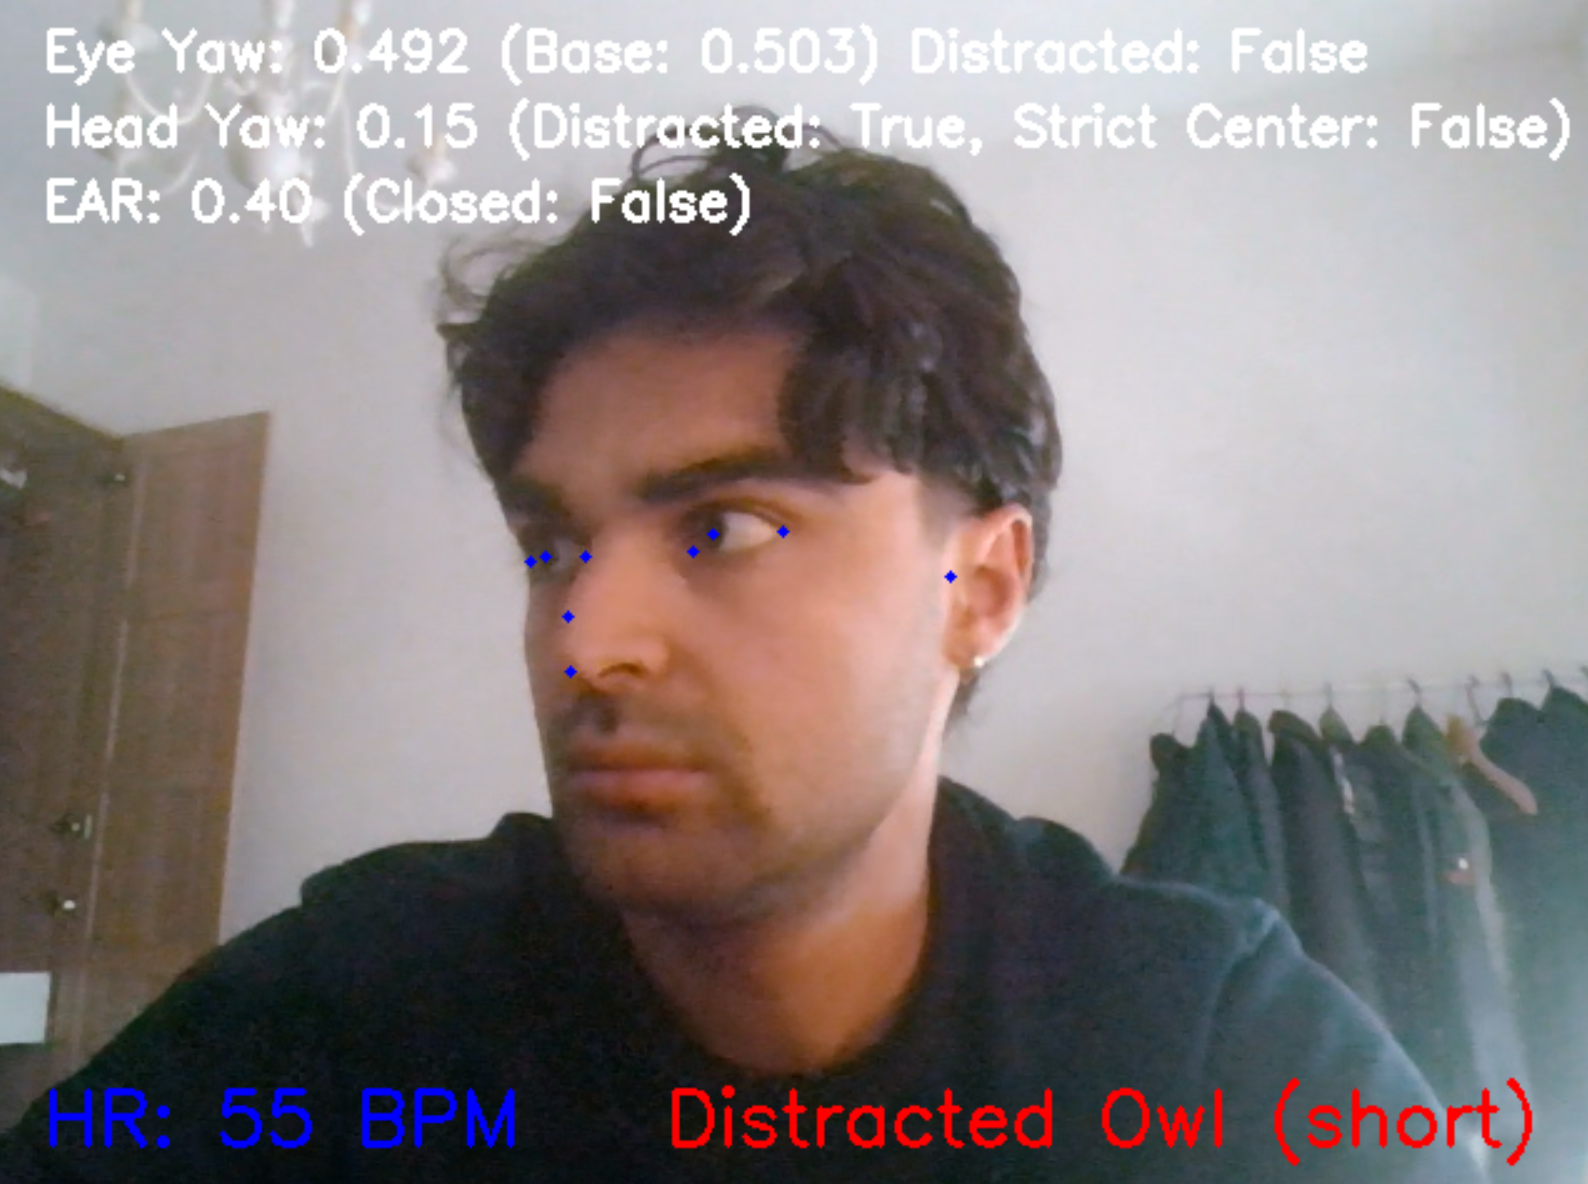
\includegraphics[width=0.42\textwidth]{images/distracted_owl_short.png} &
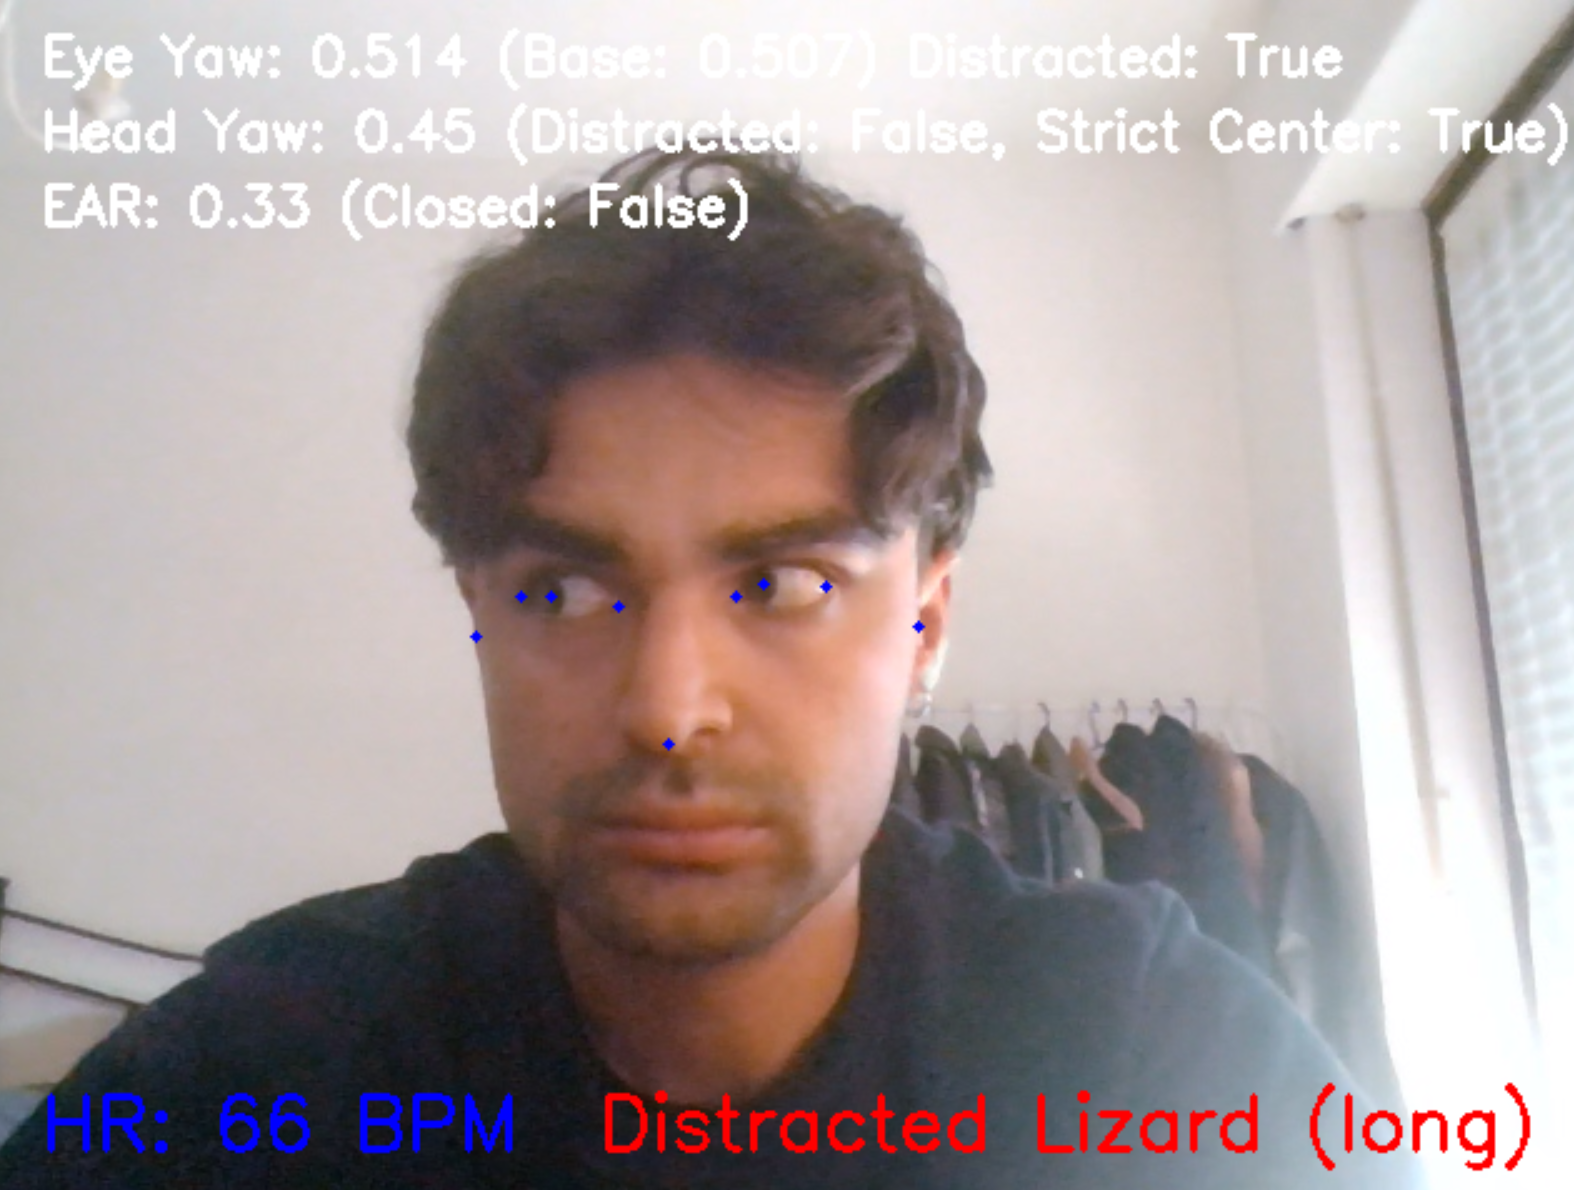
\includegraphics[width=0.42\textwidth]{images/distracted_lizard_long.png} \\
\small Distracted Owl (short) & \small Distracted Lizard (long) \\
\midrule
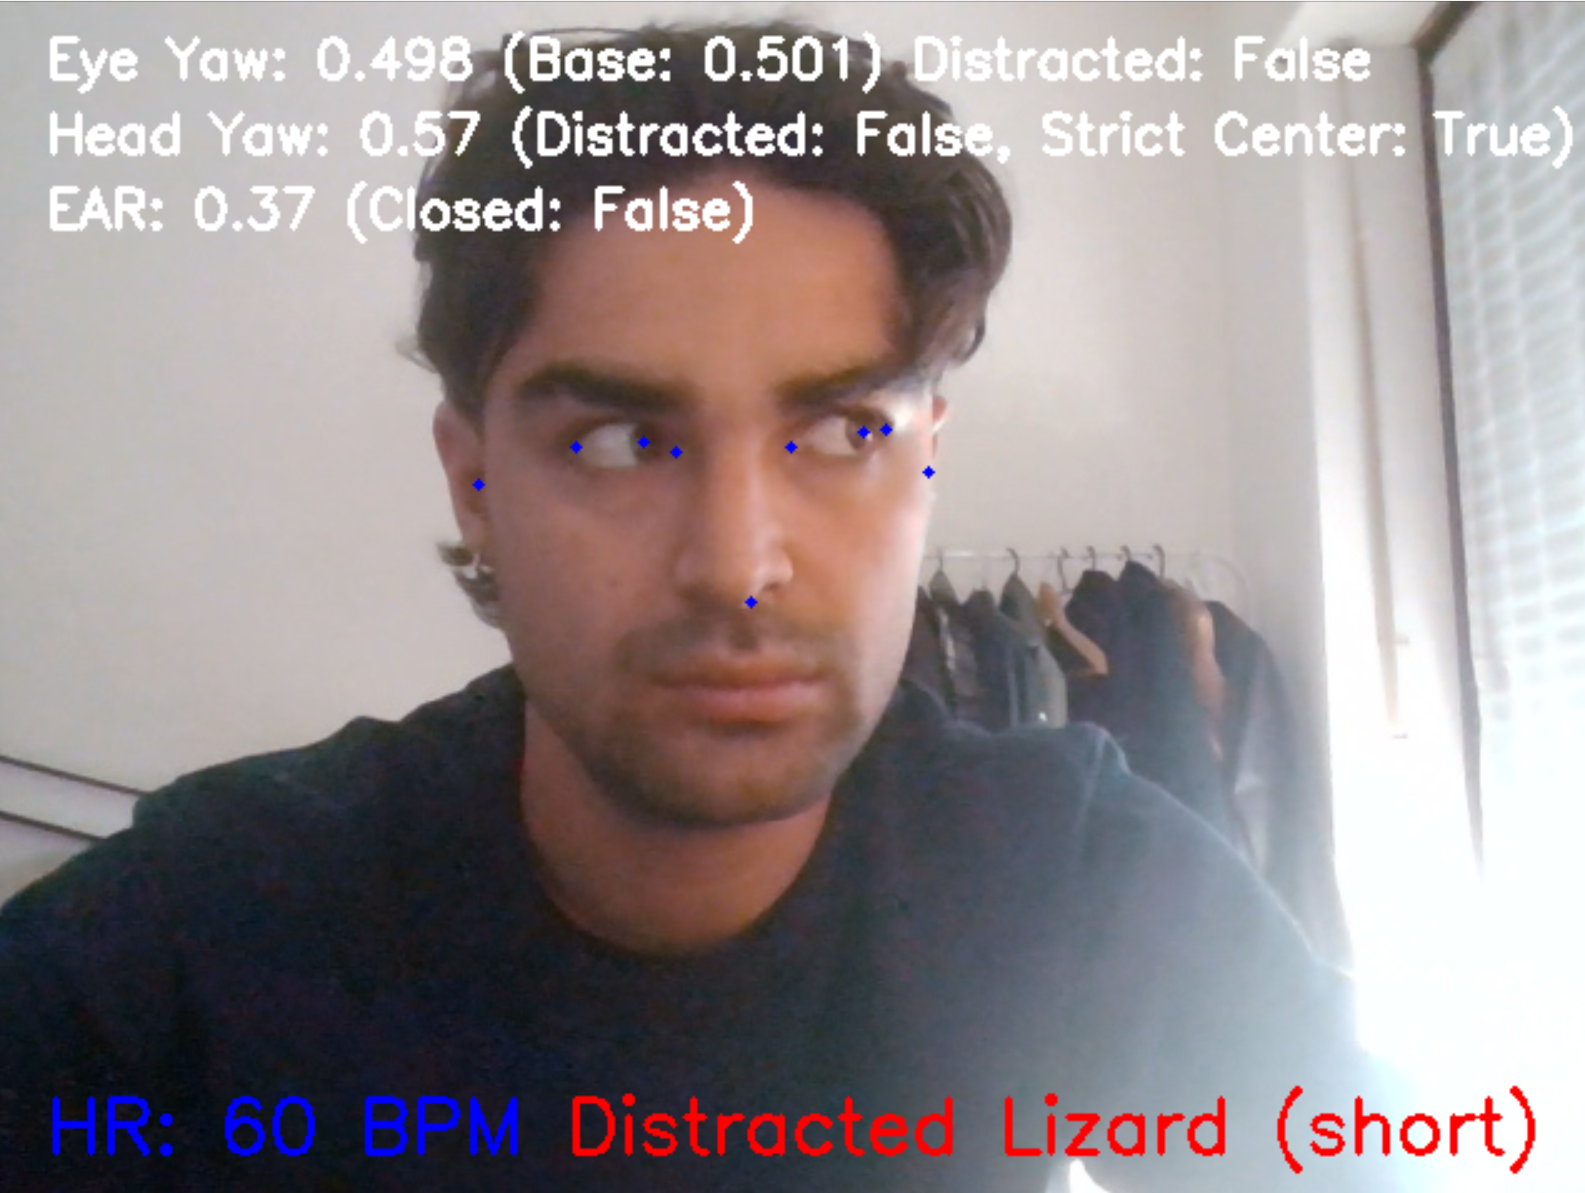
\includegraphics[width=0.42\textwidth]{images/distracted_lizard_short.png} &
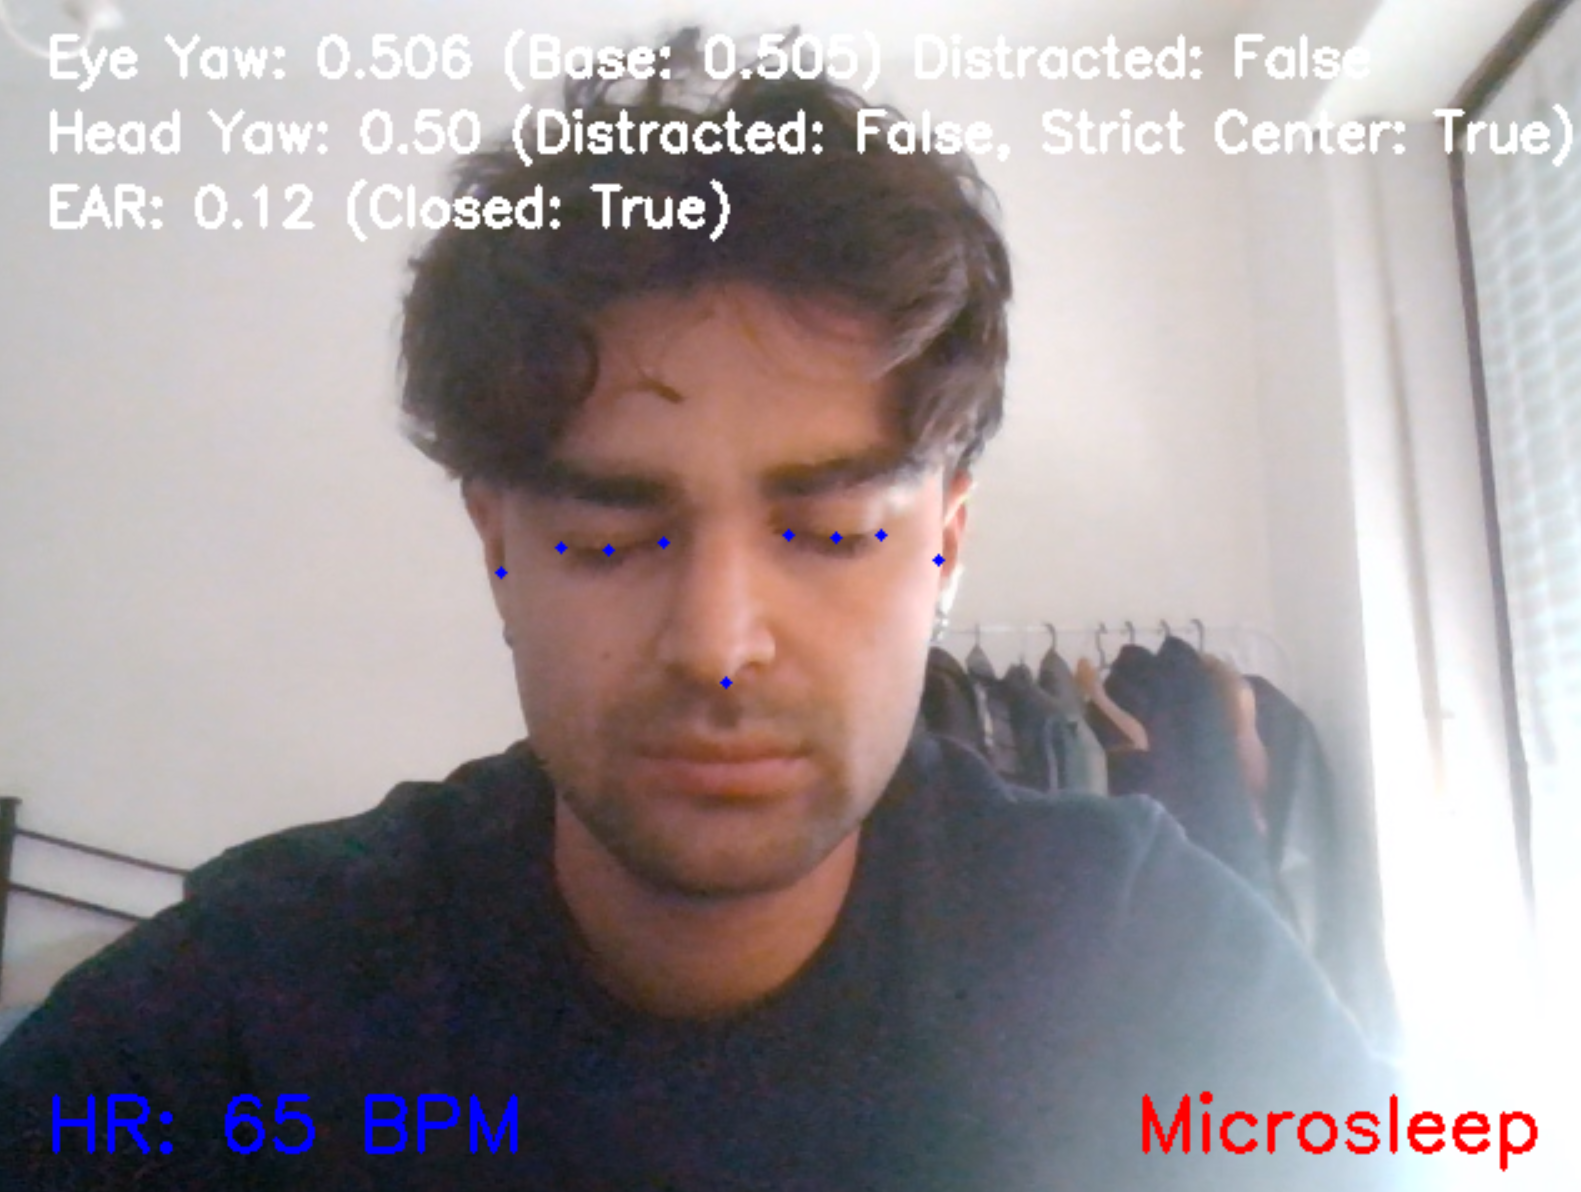
\includegraphics[width=0.42\textwidth]{images/microsleep.png} \\
\small Distracted Lizard (short) & \small Microsleep \\
\midrule
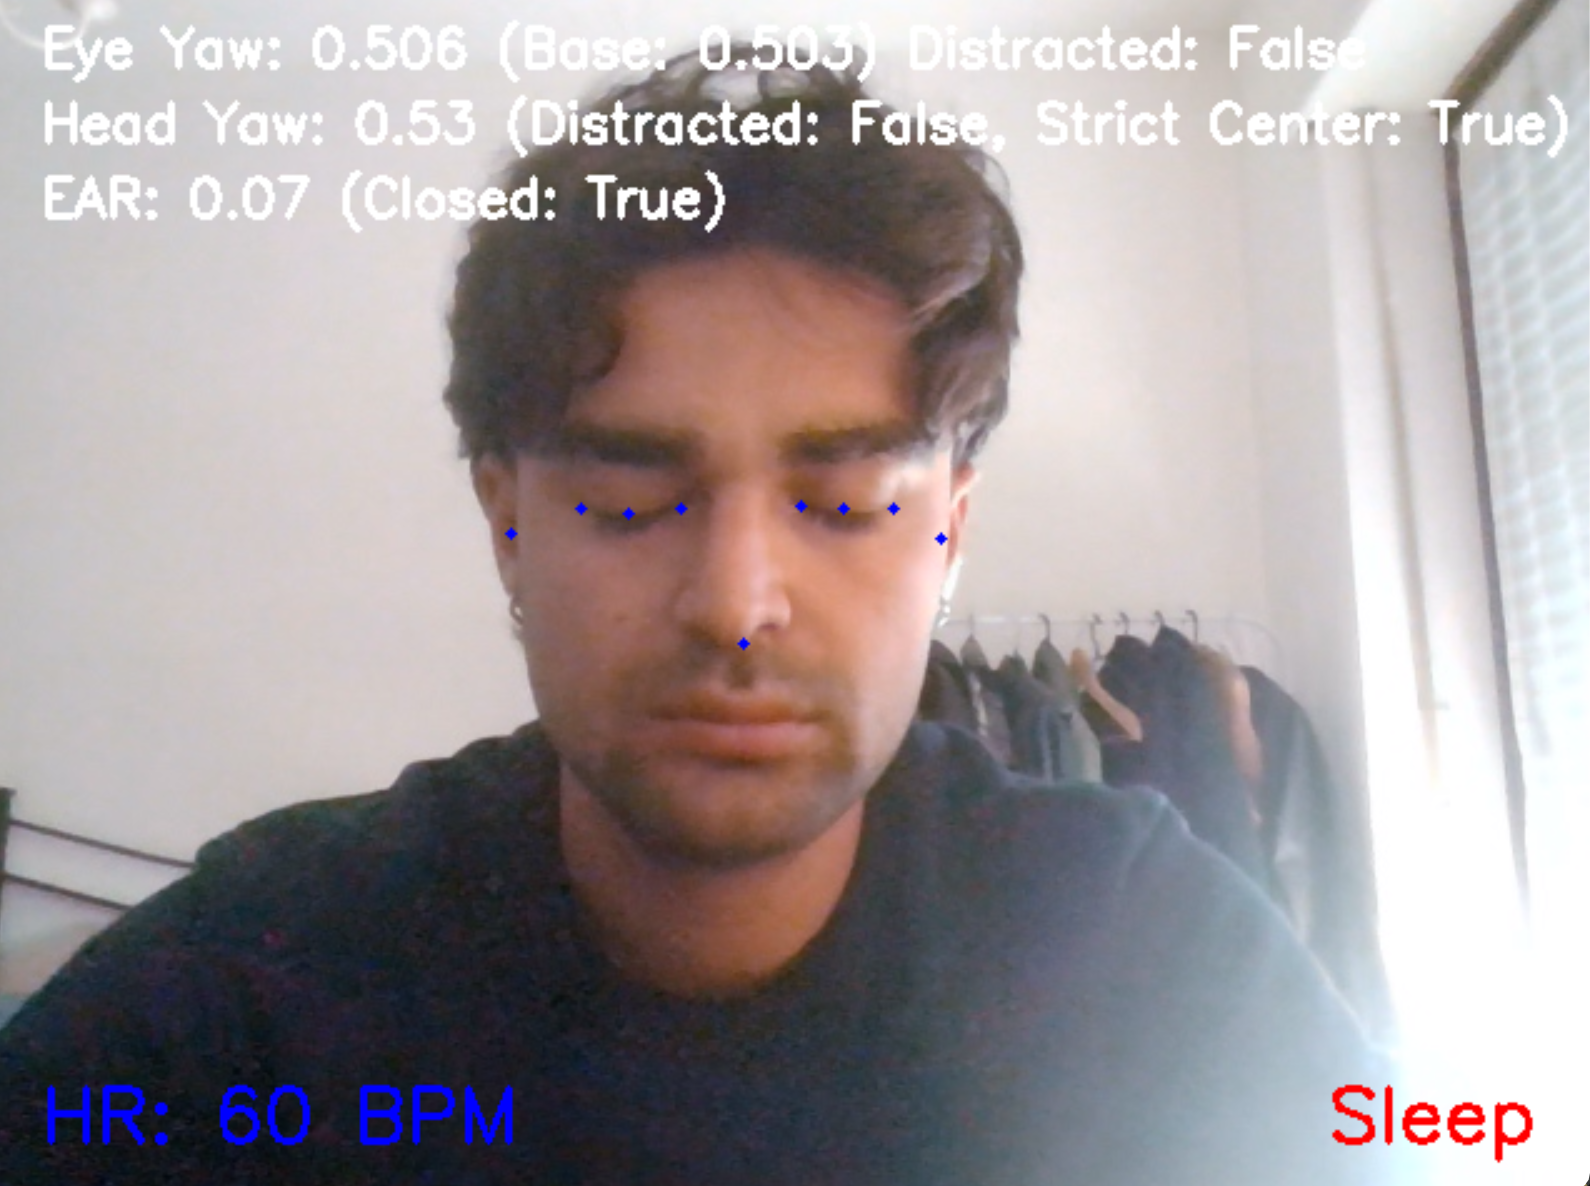
\includegraphics[width=0.42\textwidth]{images/sleep.png} &
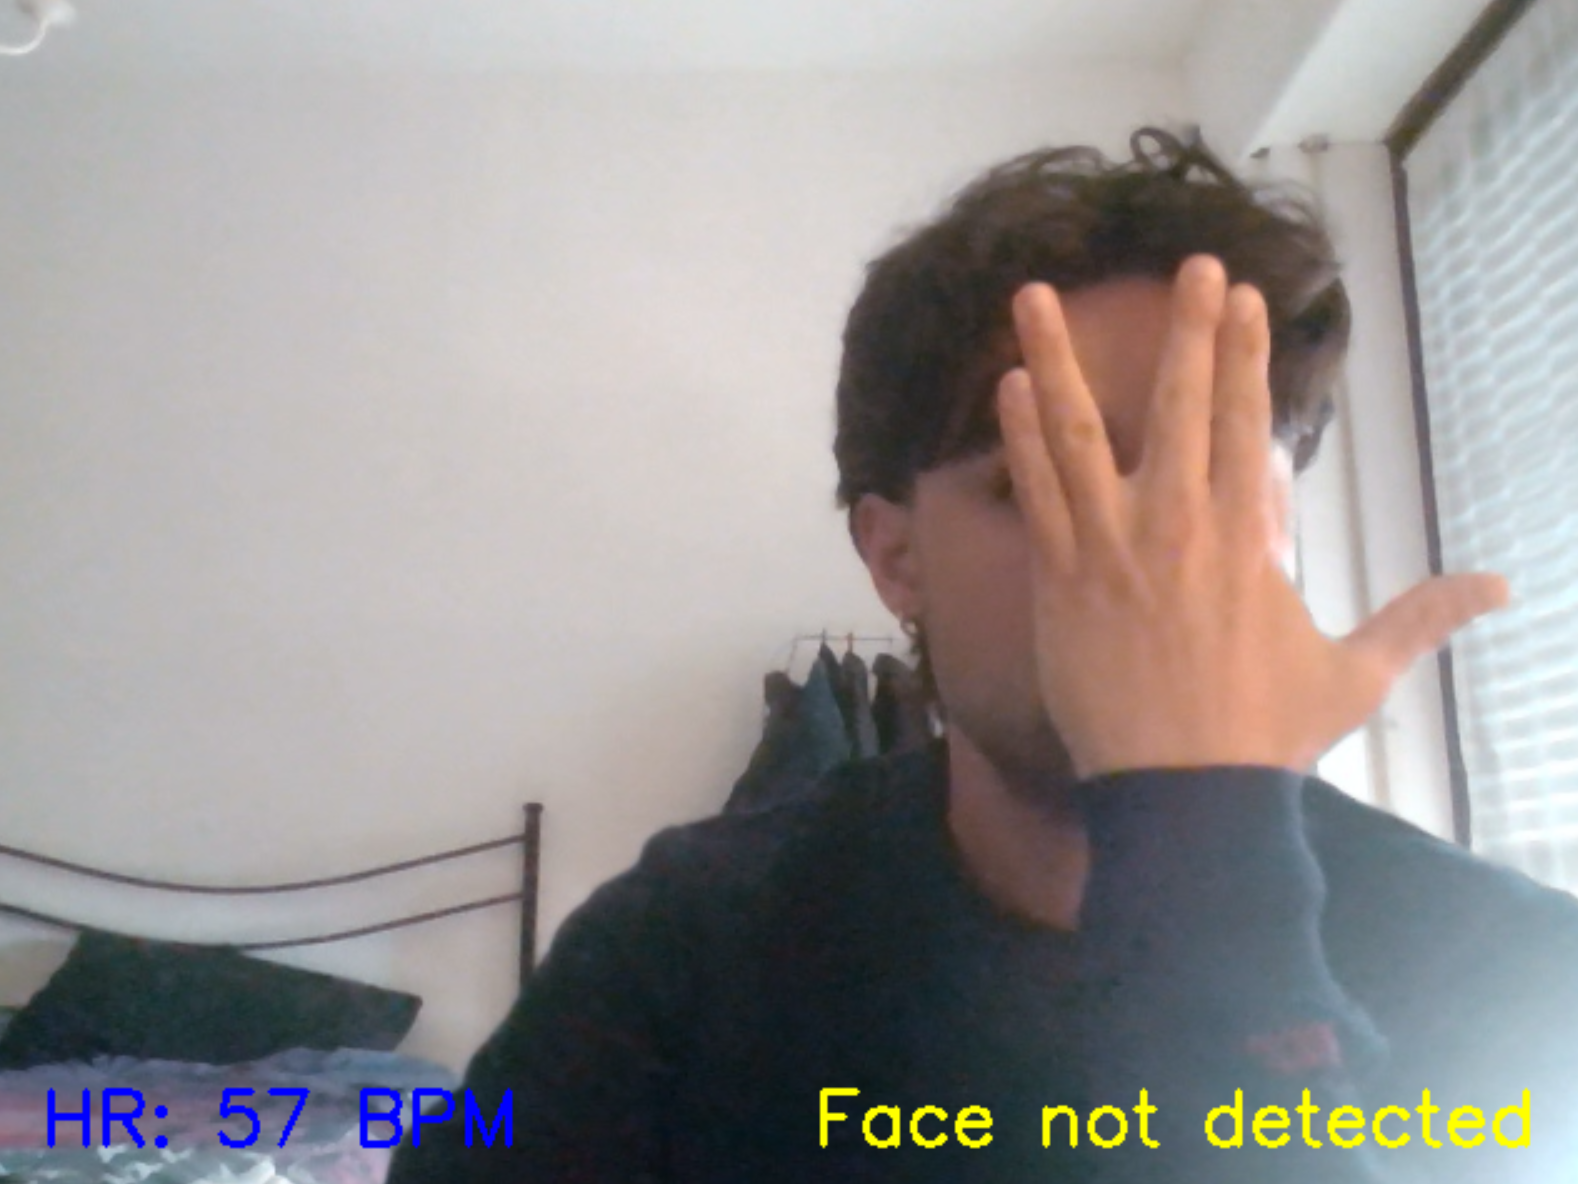
\includegraphics[width=0.42\textwidth]{images/not_face_detected.png} \\
\small Sleep & \small Face not detected \\
\bottomrule
\end{tabular}
\end{table}

% ============================================================
% 5. EXPERIMENTAL RESULTS AND DISCUSSION
% ============================================================
\section{Experimental Results and Discussion}\label{sec:experiments}

\subsection{Distraction Detection Performance}

The system was evaluated qualitatively by performing each distraction scenario multiple times and observing the system response. The key findings are:

\begin{itemize}
    \item \textbf{Owl distractions}: The head yaw ratio proved to be a highly reliable indicator of head rotation. The smoothed signal correctly tracked intentional head turns while ignoring minor involuntary movements. The long owl distraction triggered consistently after 5 seconds of sustained head rotation, and the short owl correctly accumulated time over the 30-second window.
    
    \item \textbf{Lizard distractions}: Detecting eye-only gaze shifts was considerably more challenging due to the small magnitude of iris displacement relative to head movement. The dynamic baseline calibration was essential: without it, even a slight offset in the neutral iris position (due to camera angle or lighting) would cause persistent false positives or negatives. The strict head-centre requirement ($|r_{\text{head}} - 0.5| < 0.10$) prevents the system from conflating head movements with iris movements.
    
    \item \textbf{Microsleep and Sleep}: The EAR-based eye closure detection was the most reliable feature. The 0.5-second debounce on the ``eyes open'' timer prevented brief noise spikes from falsely clearing the drowsiness state. The 2-second clearance requirement ensures that the driver has genuinely woken up before the warning is dismissed.
\end{itemize}

\subsection{Heart Rate Estimation}

The rPPG-based heart rate estimation provided plausible readings in the range of 60--90\,BPM under controlled lighting conditions. However, performance degraded noticeably under the following conditions:

\begin{itemize}[noitemsep]
    \item \textbf{Excessive head movement}: large head rotations alter the visible skin area and introduce motion artefacts that ICA cannot fully separate.
    \item \textbf{Poor or varying illumination}: the subtle colour changes due to blood volume pulsations are overwhelmed by illumination fluctuations.
    \item \textbf{Low frame rate}: a frame rate below 20\,fps reduces the Nyquist frequency, potentially aliasing the cardiac signal.
\end{itemize}

Despite these limitations, the system provides a useful estimate under typical webcam conditions and updates the display every second, consistent with the assignment requirement.

\subsection{Robustness Measures}

Several robustness mechanisms were implemented:

\begin{enumerate}[noitemsep]
    \item \textbf{EMA smoothing} on all feature signals to suppress frame-to-frame noise.
    \item \textbf{Dynamic baseline calibration} for the iris yaw ratio, adapting to individual differences.
    \item \textbf{Debouncing} (0.5\,s minimum forward-gaze duration) to prevent noise from resetting distraction timers.
    \item \textbf{History clearing} after short distraction clearance to prevent immediate re-triggering.
    \item \textbf{Priority-based state display} to ensure the most critical state is always shown.
\end{enumerate}

% ============================================================
% 6. CONCLUSIONS
% ============================================================
\section{Conclusions}\label{sec:conclusions}

This report presented a real-time Driver Monitoring System implemented in Python using MediaPipe Face Mesh for facial landmark detection and a FastICA-based rPPG pipeline for heart rate estimation. The system successfully fulfils all mandatory requirements specified in the assignment:

\begin{itemize}[noitemsep]
    \item Long and short owl distraction detection based on head yaw ratio.
    \item Microsleep and sleep detection based on the Eye Aspect Ratio.
    \item Real-time heart rate display via remote photoplethysmography.
    \item Live video output with state and heart rate overlays in the specified positions.
\end{itemize}

Additionally, both optional features were implemented:
\begin{itemize}[noitemsep]
    \item Long and short lizard distraction detection using iris tracking with dynamic baseline calibration.
\end{itemize}


Key engineering contributions include the adoption of EMA filtering for signal smoothing, dynamic baseline calibration for robust iris tracking, and a debounced state machine that prevents noise-induced false transitions. These design choices were motivated by the practical challenges encountered during development and tested empirically to achieve reliable performance under typical webcam conditions.



\end{document}
